\documentclass[a4paper]{article}
\usepackage[utf8]{inputenc}
\usepackage{fullpage}
\usepackage{amsmath,amssymb}
\usepackage[colorlinks]{hyperref} % use colored text in stead of ugly boxes
\usepackage[toc]{multitoc} % Nice two-column TOC

\usepackage{pgf}
\usepackage{tikz}
\usepackage{pictures/tikz-uml}

\usepackage{enumerate}
\usepackage{multirow}

% new line after paragraph title.
\makeatletter
\renewcommand\paragraph{\@startsection{paragraph}{4}{\z@}%
  {-3.25ex\@plus -1ex \@minus -.2ex}%
  {1.5ex \@plus .2ex}%
  {\normalfont\normalsize\bfseries}}
\makeatother


\title{Programming Life - Architectural Design }

\author{Group 5/E:\\
Felix Akkermans \\
Niels Doekemeijer \\
Thomas van Helden \\
Albert ten Napel \\
Jan Pieter Waagmeester}

\begin{document}
\maketitle

\vfill

\small{\tableofcontents}
\pagebreak
\section{Introduction}
\subsection{Purpose of the System}
The purpose of our system is to create a modeling environment for biology experts and people who work in the field of genetics. Within this modeling environment, you can easily model BioBricks. BioBricks are biological gates, which are created by gene manipulation. Our system should be able to create BioBricks with basic components, like AND and NOT gates. The system should also be able to import and export BioBricks, making it possible to create larger constructions with earlier designed BioBricks.

\subsection{Design Goals}
Our design goal for this project is to successfully implement the system mentioned above. We aim to make the system easy to use for people without too much knowledge of computers.
%We aim to make the system easy to use for people without too much knowledge of computer science.

\subsection{Definitions, acronyms and abbreviations}
\begin{description}
	\item[BioBrick] is the key word in this project. A BioBrick is a logical gate representation of a manipulated cell. The idea behind this is: Genes can be manipulated to work as gates. By doing this we can create logical structures using cells. A BioBrick is a model for this. The term Bio comes from Biology. The term Brick comes from the idea that these BioBricks should be building blocks for a larger system. With BioBricks you can build bigger structures. 
	\item[Client-side] is the part of the program which takes place on the computer of the client/user. The opposite is server-side. For our program, the client-side is a GUI implemented in JavaScript. 
	\item[Server-side] is the part of the program which takes place on the server. In our case it is implemented in Java. This part will do the heavier computations, so the client-side only has to display the results.
	\item[GUI] is a Graphical User Interface. This is the part of the program which you actually see as a user. It is the screen which shows you the program and allows you to do things. 
	\item[JSON] (JavaScript Object Notation) is a lightweight data-interchange format. It is easy for humans to read and write. It is easy for machines to parse and generate.
	\item[AJAX] (Asynchronous JavaScript and XML) is a technique in which data can be exchanged between client and server side. This can be done asynchronously, meaning your main program does not have to wait for the results of the data transaction before it can continue. We will use this as a part of our communication between our JavaScript client-side and our Java server-side.
	\item[SBML] is a Markup Language specially designed for Synthetic Biology. We will use this to simulate BioBricks. An external SBML solver application will be used for simulating the BioBricks.\\

	\item[MVC] stands for Model View Controller. It is an architectural structure which separates the display(View) of the program from the input/output handling(Controller) and the data representing part(Model). By doing this your application remains structured, can be tested in separate parts and is easier to maintain or change.
\end{description}

\subsection{References}
\begin{description}
	\item[\url{http://www.json.org/}] The JavaScript Object Notation.
	\item[\url{http://www.sbml.org/}] The Systems Biology Markup Language
\end{description}

\subsection{Overview}
So this chapter was all about what we wanted to achieve globally. We want to create a modeling environment for biologists and genetics experts to model BioBricks. These BioBricks represent genetically modified cells or genes which act as logical gates. The Definitions section explains some of the major concepts. The full architectural design will be explained in detail how we intend to implement everything.

\section{Proposed software architecture}
\subsection{Overview}
In this chapter we will discuss the exact architectural design of our application. We will go into detail about how the system is build up. There will be a short explanation of every sub-system. This will all be done in chapter~2.2. There is a mapping of how different parts of our application interact with each other in chapter~2.3. In 2.4 there will be an explanation of how we manage data. Where and how will we save our BioBricks? Which format will we use? These are all questions we will answer. In chapter~2.5 we will tell something about how the application handles global recourses. There we will also explain why we chose not to have a complex access structure. Concurrency, how communication is handled in our system, will be discussed in chapter~2.6. Finally we will discuss the boundaries of our system. Where does our system end and what happens in case of errors or crashes? 

\subsection{Subsystem Decomposition}
The main decomposition in our system is the devision between the client and the server. The server is responsible for file operations and the more heavy calculations, while the client is mainly just a GUI. A schematic view of this decomposition can be found in figure~\ref{fig-decomposition}. In rest of this section we'll discuss each interaction in more detail.

\begin{figure}[h!]
	\caption{The system decomposition}
	\label{fig-decomposition}
	\centering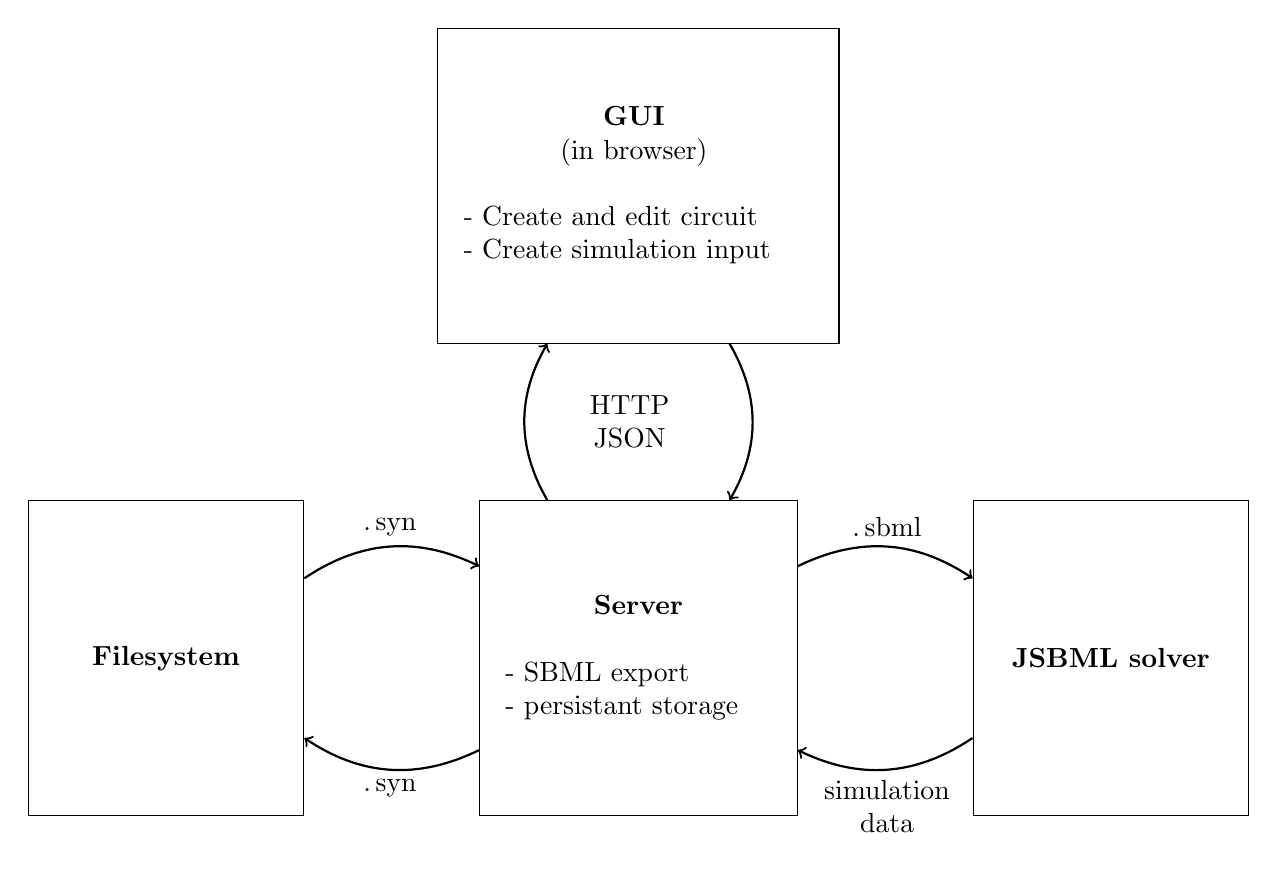
\begin{tikzpicture}
	\tikzstyle{part}=[rectangle, minimum height=4cm, minimum width=3.5cm,draw=black]
	\node[part] (server) at(0,0) {
		\begin{tabular}{ll}
			\multicolumn{2}{c}{\textbf{Server}} \\
			\\
			- SBML export & \\
			- persistant storage & \\
		\end{tabular}
	};
	
	\node[part, align=center] (client) at( 0, 6) {
		\begin{tabular}{ll}
			\multicolumn{2}{c}{\textbf{GUI}} \\
			\multicolumn{2}{c}{(in browser)} \\
			\\
			- Create and edit circuit & \\
			- Create simulation input \\
		\end{tabular}
	};
		
	\node[part] (jsbml) at(6,0) {\textbf{JSBML solver}};

	\node[part] (filesystem) at(-6, 0) {\textbf{Filesystem}};
	
	\path[->, thick, bend left]
		(server) edge node[right=.7cm,align=center] {HTTP \\JSON} (client)
		(client) edge (server)
		(jsbml) edge node[below, align=center] {simulation\\ data} (server)
		(server) edge node[above] {.\,sbml} (jsbml)
		(filesystem) edge node[above]{.\,syn} (server)
		(server) edge node[below]{.\,syn}  (filesystem);
	
\end{tikzpicture}
\end{figure}

\pagebreak

\subsubsection{Interface (API) of each sub-system}

\paragraph{Persistent storage}
User generated circuits will be stored in simple text files. Since the communication between the client and the server is in JSON already, it is convenient to use that format for persitent storage aswell. The format will include:
\begin{enumerate}[-]
	\item The circuit as a directed graph,
	\item Protein assignments for each edge,
	\item Position information for each elemental gate,
	\item Grouping information to support user generated `gates'\footnote{As discussed in requirement 1, see RAD.}.
\end{enumerate}

\paragraph{SBML export}
Since SBML is an available standard and differential equation solvers exist for this format, we'll use it to run the simulation. The circuit will be represented in SBML and imported in the solver. The solver will respond with calculated concentrations of different species\footnote{SBML-term for different signals in the simulation} as a function of time.

\paragraph{HTTP interface} 
We propose the following API for the server-side of our application. Every model is represented by an object which stores the needed information. It is basically a directed graph with building blocks as nodes. \\
\begin{description}
	\item[listFiles(): list of filenames] -
		Returns a list of available models.\\
		If there are no available files, then it returns an empty list.
	\item[getFile(fileName): model] -
		Returns the BioBrick model stored in fileName.\\
		If the file does not exist or if the file is corrupt, it will give an error.
	\item[putFile(fileName, model)] -
		Stores model in a file called fileName.\\
		If something goes wrong while saving, it will give an error.
	\item[listProteins(): list of proteins] -
		Returns a list of proteins, including their meta-data.\\
		With absence of information, it will give an error.
	\item[listModels(): list of models] -
		Returns a list with a model for all available files.\\
		Returns an empty list when there are no available files.
	\item[modelToSBML(model, fileName)] -
		Exports model to an SBML file and saves it to a file called fileName.\\
		Returns an error if model is not a valid model.\\
		Returns an error if saving failed. \\
	\footnote{\textbf{SBMLToModel} seems a logical counterpart, but because SBML is such a low level format, not all the information required to rebuild the model can be extracted. Therefore we will not implement it}
	\item[simulate(fileName, inputValues): outputValues] -
		Simulates the SMBL model saved in fileName with given input values and returns the matching outputvalues.\\
		Returns an error if the simulation of the file failed.
	\item[validate(model): boolean] -
		Validates the model and returns true if model has everything defined to simulate it, and returns false otherwise.\\
\end{description}

For the client-side of our application, we will not follow a predefined API. As the client will only implement the view part of the model, view controller (MVC) system, it will only reuse the API of the server and not implement an API of its own. The server will respond to the API calls with a standard JSON object, as proposed in figure~\ref{fig-jsonDefault}. The response always contains a success field. When the server cannot respond with success, the reason will be given in the message field. In case of a response with data, the client can find it in the data field of the servers response. \\

\begin{figure}[h!]
\caption{Some examples of JSON responses in a generic wrapper}
\label{fig-jsonDefault}
{\footnotesize
\begin{tabular}{p{4.3cm} p{4.3cm} p{4.3cm}}
	%empty row
\\
	Generic response: &
	Response of getFiles(): &
	Response for getFile(fileName) for a non-existing file: \\
\begin{verbatim}
{
  "success": boolean,
  "message": <string>,
  "data": <object>
}
\end{verbatim}

&

\begin{verbatim}
{
  "success": true,
  "message": "",
  "data": {
    "files": [
      "example1.syn",
      "d-flipflop.syn",
      "xor-gate.syn"
    ]
  }
}
\end{verbatim}

&

\begin{verbatim}
{
  "success": false,
  "message": "Requested file not found.",
  "data": {}
}
\end{verbatim}
\\
\end{tabular} }

\end{figure}

\pagebreak
\pagebreak

\subsection{Hardware/Software Mapping}
Our architecture is composed of two major elements, the client implemented as a web application and the server, implemented as a Java servlet on top of Apache Tomcat. The browser has to be Chrome~15+ or Firefox~7+, the supporting system hardware and operating system is not relevant. The server can be run on the same machine, which will be the case during the development stage. When the server and the client are not on the same machine, a reliable network connection has to be available.

%&latex
\subsection{Persistent Data Management}
The application will persistently store data serverside on the disk. A database seems overkill for the rudimentary data storage that is required, and the already existent and mature text formats are good candidates to save our data in. The application will store data using the following files:
\begin{enumerate}
\item \textbf{.xml (SBML)} \\
A \verb=text/xml= file in the Systems Biology Markup Language schema that describes the abstract model of the biological system. Within the domain of our application it will primarily be used to describe the biological processes of a modeled circuit/BioBrick.

\item \textbf{.sym (JSON)} \\
A \verb=text/json= file in our made up extension
that embodies the entire modeled circuit/BioBrick in JavaScript Object Notation. The object structure has to comply with that of the application to be read.\end{enumerate}

\subsection{Global Resource Handling and Access Control}
The application will be controlled through a web interface. As is dictated in the requirements, the application will only work will a single user at a single point in time, and there is no access control implemented. A browser will connect to the server and without authorization will be able to access the functionality. The decision on this was made because the focus should be on implementing the required functionality. We agreed that security and multi-user operation would be a nice-to-have, but to ambitious with the current goals in mind.

This means that in theory anyone who has access to the network where the server runs could operate the application, so users of the application should be aware that they do not work on and/or save sensitive information.

\subsection{Concurrency}
As is described in the previous section, our system will not support multi-user operation, so operation is only guaranteed for one client-server connection at the same time. This reduces concurrency issues, but leaves some scenarios to be thought about. Because user interaction is a dominant part of our application, concurrency problems may not hinder the workflow or be very problematic. This implies multi-threading, and the following subsystems will have to run on a separate thread with concurrency handling:

\begin{enumerate}
\item \textbf{Main controller} \\
The main controller will have to be able to handle calls from multiple subsystems at the same time. For example the user must still be able to interact with the server when the server is reading/writing a lengthy XML file.\item \textbf{HTTP request handler} \\
See next item.
\item \textbf{Web server} \\
These two subsystem must be able to terminate when hung in the processing of a HTTP request or serving HTTP to a client. Therefore it must be isolated in a separate thread. Also if we decide to implement multi-user support this would be a lot easier to implement as we could easily start multiple of these threads. 
\item \textbf{XML parser/writer} \\
This subsystem must also be able to terminate when hung without crashing the rest of the server.
\item \textbf{Simulation math} \\
This subsystem must also be able to operate independently of the rest of the server systems so in case lengthy simulations are performed, the server can still interact with the client and the simulation can be aborted.
\item \textbf{GUI} \\
This is essentially the browser, and in this sense should also be considered a separate thread. This has the benefits as described in the system decomposition. Because we only support recent versions of the major browsers concurrency problems with the GUI are already covered.\end{enumerate}
%\subsection{Persistent Data Management}
%(file/ database, database design)
%\subsection{Global Resource Handling and Access Control for the different actors}
%\subsection{Concurrency}
%(which processes run in parallel, how do they communicate, how are deadlocks prevented?)

\subsection{Boundary Conditions}
%~ (how is the system started and stopped, what happens
%~ in case of a system crash)

In a deployment context, the server will run somewhere on a server indefinately. At any point, the user can start a browser on a random device and start to use it.
During the development stage, the server will run locally, and has t be started by the user before the user can start using it.
The user's work will be saved at regular time intervals to prevent loss of work in case of a browser crash.

\end{document}
